%%%%%%%%%%%%%%%%%%%%%% Props %%%%%%%%%%%%%%%%%%%%%%
\documentclass{article}

\usepackage[french]{babel}
\usepackage[utf8]{inputenc}
\usepackage[T1]{fontenc}
\usepackage{graphicx}
\usepackage{fancyhdr}
\usepackage{eurosym}
\usepackage{color}
\usepackage{soul}
\usepackage{listings}
\usepackage{enumitem}
\usepackage{enumerate}

\pagestyle{fancy}
\lhead{Soutenance 3}
\chead{Deadly Science}
\rhead{Custos Carceris}

\definecolor{mygreen}{rgb}{0,0.6,0}
\definecolor{mygray}{rgb}{0.5,0.5,0.5}
\definecolor{mymauve}{rgb}{0.58,0,0.82}

\lstset{ 
  commentstyle=\color{mygreen},
  keywordstyle=\color{blue},       % keyword style
  numberstyle=\tiny\color{mygray}, % the style that is used for the line-numbers
  rulecolor=\color{black},         % if not set, the frame-color may be changed on line-breaks within not-black text (e.g. comments (green here))
  stringstyle=\color{mymauve},     % string literal style
  language=[Sharp]C,                 % the language of the code
  backgroundcolor=\color{white},   % choose the background color; you must add \usepackage{color} or \usepackage{xcolor}; should come as last argument
  basicstyle=\footnotesize,        % the size of the fonts that are used for the code
  breakatwhitespace=true,         % sets if automatic breaks should only happen at whitespace
  breaklines=true,
  extendedchars=true,              % lets you use non-ASCII characters; for 8-bits encodings only, does not work with UTF-8
  frame=single,	                   % adds a frame around the code
  tabsize=2,	                   % sets default tabsize to 2 spaces
  showstringspaces=false,
  numbers=left,
}

\begin{document}


%%%%%%%%%%%%%%%%%%%%%% Titre %%%%%%%%%%%%%%%%%%%%%%
\begin{titlepage}
	\centering
	{\scshape\LARGE Custos Carceris\par}
	\vspace{1cm}
	{\scshape\Large Rapport de projet\par}
	\vspace{1.5cm}
	{\huge\bfseries Deadly Science\par}
	\vspace{2cm}
	
\includegraphics[width=0.5\textwidth]{logo.png}\par\vspace{1cm}
	{\Large\itshape Léandre Perrot\par}
	{\Large\itshape Yann Boudry\par}
	{\Large\itshape Steve Suissa\par}
	{\Large\itshape Célian Raimbault\par}
	\vfill
	Un projet EPITA
	\vfill
	{\large \today\par}
\end{titlepage}



\newpage
\tableofcontents


%%%%%%%%%%%%%%%%%%%%% Intro %%%%%%%%%%%%%%%%%%%%%%

\newpage
\section{Introduction}
Depuis le début de l'année, notre groupe a travaillé sur ce projet, qui est aujourd'hui fini et complet. De plus nous avons pu rajouter bien plus de choses que le cahier des charges demandait, c'est-à-dire :

\begin{itemize}
\item Un second mode de jeu nommé le mode Nocturne, où toutes les lampes du laboratoire sont éteintes et où le joueur ne peut voir que grâce à sa lampe torche,
\item un système de paramètres de la partie permettant de choisir:
\begin{itemize}
\item la taille du labytinthe parmis plusieurs tailles prédifinies, où en choisisant une taille personnallisée,
\item le nombre de joueurs dans la partie
\item et le mode de jeu.
\end{itemize}
\item une cinématique dans le menu principal,
\item une refonte graphique totale des menus pour mieux coller à l'atmosphère du jeu et pour un meilleur rendu visuel, 
\item plus de 20 œufs de pâques cachés dans le jeu,
\item plus de 13 objets différents et bien plus!
\end{itemize}

Evidemment tout cela sera expliqué par la suite. On notera que nous n'avons pas été en retard durant toute la durée du projet, car les seules choses sur lesquelles on était légèrement en retard était largement comblé par le reste.

Nous sommes très fiers et confiants en notre projet. D'ailleurs nous allons le continuer pendant les vacances d'été tellement que nous y sommes attachés. Ce fut un immense défi, que ce soit parce que il diffère largement d'un jeu de labyrinthe lambda, ou que ce soit pour la programmation car il nous a fallut comprendre et utiliser de nouveaux outils comme Unity ou Photon. Il a aussi fallu tout synchroniser en réseau, en plus que nous avons voulu faire un réseau plus large que nécessaire.

Le projet fut déjà grandement crée lors des deux premières soutenances, ces derniers mois n'ont servis qu'a peaufinné le tout, résoudre des bugs...

D'ailleurs pour réduire le plus de bugs, on a décidé de regrouper plus de 8 testeurs sur notre jeu en version alpha que l'on a réuni sur un salon dédié.

\newpage
\section{Reprise du cahier des charges}
\paragraph{Caméra}
Chaque joueur doit avoir une caméra, elle doit représenter un angle de vue humain de 180 degrés. Elle doit donc prévenir et arrêter les mouvement de caméra impossible pour un humain comme par exemple pouvoir regarder derrière la tête.

\paragraph{Déplacements}
Chaque joueur doit pouvoir se déplacer dans toutes les directions. Il faut pouvoir facilement changer les vitesses, frictions en fonction de l'avancement du projet. Il peut aussi donner des coups de poing, qui baissent la barre d'endurance du joueur en face.

\paragraph{Endurance}
Les joueurs ont au dessus de leur tête leur pseudo, coloré en fonction de leur statut, et une barre d'endurance qui descend en fonction des dommages encaissés. Lorsque celle-ci est vide, le joueur avance plus lentement et la barre devient grise et se recharge progressivement. 

\paragraph{Statuts}
Lorsqu'un joueur est corrompu, il faut voir si un joueur guéri n'est pas trop près de lui, sinon lui aussi devient corrompu et doit aller contaminer les autres joueurs.

\paragraph{Phases}
Lorsque tous les joueurs sauf un ont ramassé les sérums, la deuxième phase du jeu doit commencer. Le dernier joueur doit devenir corrompu et il faut aussi s'assurer que tous les joueurs soient soit guéri, soit corrompu, soit invisible. La partie doit se terminer lorsque tous les joueurs sont infectés, et l'on doit afficher un écran de victoire si l'on gagne, et un écran de défaite si ça n'est pas le cas.

\paragraph{Sérums}
Les joueurs peuvent être pris par les joueurs pour se guérir. Il faut faire attention à ce qu'un joueur corrompu ou guéri ne puisse pas prendre de sérum, et que les sérums sont bien détruits lorsqu'ils sont ramassés. Il faut aussi faire attention pour qu'il y ait exactement le bon nombre de sérums dans le labyrinthe, c'est-à-dire le nombre de joueurs moins 1.

\paragraph{Labyrinthe}
Le jeu doit contenir un labyrinthe assez grand pour se pouvoir se perdre. Il faut aussi mettre plusieurs salle différentes pour un meilleur gamplay et pour mieux se perdre. Chaque salle doit avoir des meulbles divers spécifiques, avec des modèles diffénrents. Il doit être généré aléatoirement de manière à ce qu'on est un labyrinthe différent quasiment à chaque fois que l'on crée une nouvelle partie. Il faut aussi faire attention que les sérums se génère à l'intérieur du labyrinthe.

\paragraph{Modèles}
Chaque composants du labyrinthe doit avoir un modèle particulier, que ce soit les joueurs, les sérums, les meubles et différents objets des salles et tous les autres objets aussi.

\paragraph{Menus}
Il faut un menu principal plus un menu pour créer la salle, la rejoindre, et la quitter. Le menu principal doit contenir un bouton pour quitter le jeu, et un bouton pour la quitter. Dans le second menu, il faut pouvoir accéder aux différents joueurs présents dans la salle puis pouvoir commencer la partie lorsque tous les joueurs sont prêts.

\paragraph{Réseau}
Le jeu doit être jouable en réseau, les effets des sérums doivent être synchronisés sur tous les joueurs, ainsi que la phase de la partie. Il faut aussi associer une caméra à chaque joueur, et faire attention qu'il y'en assez pour tout le monde, mais pas trop non plus! 

\paragraph{Site Web}
Il faut un site Web clair et net et esthétiquement plaisant à regarder. Il doit comporter les informations sur notre groupe, les liens pour télécharger les rapports de soutenance, de projet et le jeu. Il faut aussi qu'il contienne les règles et des images du jeu pour avoir une idée du jeu.

\newpage
\section{Présentation du projet}



\subsection{Menus}
blablabla
%%%%%%%%%%%%%%%%%%%%%% Yann %%%%%%%%%%%%%%%%%%%%%%%%%%%%%%
\subsubsection{Menu principal}
blablabla
\newpage
\subsubsection{Menus de connexion}
%%%%%%%%%%%%%%%%%%%%%% Steve%%%%%%%%%%%%%%%%%%%%%%%%%%%%%%
Pour se connecter il y'a trois menus, le menu pour créer la partie, le menu pour changer les paramètres de la partie, et enfin le menu on peut voir les joueurs connectés et commencer la partie. Chacun des 3 menus ont subi une refonte graphique pour correspondre à l'ambiance du jeu et avoir un aspect visuel plus plaisant.

\paragraph{Menu pour créer la partie}

Voici à quoi ce menu ressemble : 

\begin{figure}[!ht]
    \centering
    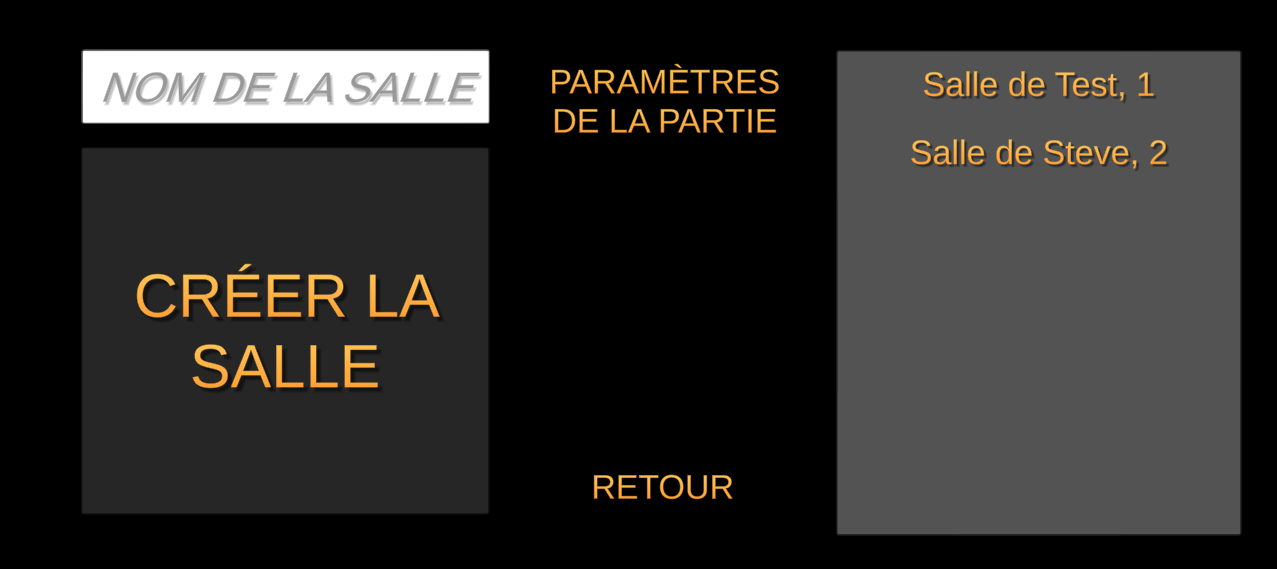
\includegraphics[width=0.8\textwidth]{Menu1.png}
    \caption{Menu pour créer la salle}
    \label{Menu pour créer la salle}
\end{figure}

Il est composé de deux parties. Celle de gauche on peut écrire dans la barre blanche le nom de la salle que l'on veut créer et un bouton "Créer la salle" qui comme son nom l'indique permet de créer la salle et d'entrer dans un autre menu que l'on verra par la suite. La partie droite liste chacune des salles avec leur noms et le nombre de joueurs déjà présents dans la salle. Elle est sur un tableau défilant ce qui permet d'avoir autant de parties que l'on souhaite. Cela permet de savoir si par exemple on va attendre plus ou moins longtemps avant le début de la partie. Pour rejoindre la salle que l'on souhaite, c'est simple, il suffit de cliquer dessus et cela nous fait rentrer dans la dite salle. A noter que si la salle est remplie à son maximum, elle ne sera pas montrée comme visible, vu qu'on ne peut pas la rejoindre. En ce qui concerne les deux boutons du milieu, le bouton "Retour" nous fait retourner à l'écran principal et le deuxième bouton nous transporte dans le menu des paramètres du labyrinthe que l'on va maintenant regarder.

\paragraph{Menu pour les paramètres de la partie}

Dans ce menu on peut changer de mode de jeu entre Classique et Nocturne (ces modes de jeu seront expliqués par la suite). On peut aussi changer le nombre de joueurs de la partie. Enfin on peut choisir la taille du labyrinthe parmis plusieurs dimensions prédéfinies ou bien choisir une taille personnalisée (par exemple un labyrinthe rectangulaire) en l'écrivant sur la barre blanche et confirmer. Pour sélectionner l'option que l'on souhaite, il suffit encore tout simplement de cliquer dessus. Par exemple sur la Figure 2, on peut voir que le mode de jeu choisi est Classique, que la salle peut contenir quatre joueurs et que la taille du labyrinthe est de dix en largeur et 10 en longueur. Lorsque l'on a choisi ses paramètres, il suffit d'appuyer sur le bouton "Retour" qui nous envoie sur le menu précédant et on peut créer la partie avec les paramètres enregistrés. On peut souligner que les modes de jeu et les tailles du labyrinthe sont sur des tableaux défilants, ce qui permet premièrement l'ajout de nouveaux modes ou de nouvelles tailles facile, mais aussi que l'on peut en ajouter autant qu'on veut, il suffit juste d'utiliser la molette de la sourie pour accéder aux options tout en bas.



\begin{figure}[!ht]
    \centering
    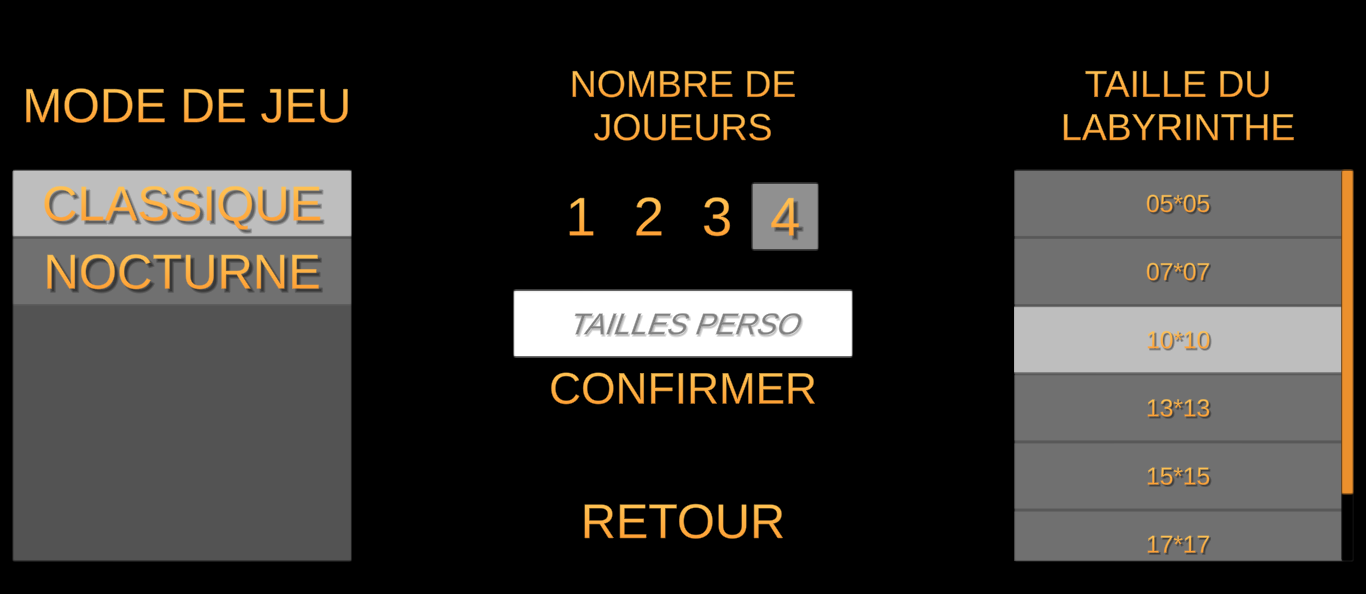
\includegraphics[width=0.8\textwidth]{Menu2.png}
    \caption{Menu pour les paramètres de la partie}
    \label{Menu pour les paramètres de la partie}
\end{figure}


\paragraph{Menu pour commencer la partie}

Ce menu a la particuliarité d'être différend en fonction de notre rôle dans la partie. Si on est l'hôte de la salle, alors le bouton en bas à gauche est "Commencer" permettant de débuter la partie, et sinon il est nommé "Prêt" qui permet de savoir si chacun des joueurs est prêt à commencer la partie comme montré sur les Figures 3 et 4. D'ailleurs à droite, on peut voir la liste des joueurs avec leur pseudonyme et leur rôle. A nôter que l'actualisation des statuts des joueurs est quasiment instantané et que le bouton "Prêt" change si on est prêt ou pas. Si on ne l'est pas il sera renommé "Non Prêt". L'hôte ne peut commencer la partie que si chacun des joueurs, et chacun des joueurs entre dans la salle avec un statut "Non Prêt". Dès que le nombre de joueurs attendus correspond au nombre de joueurs dans la salle et que tous les joueurs sont prêts, l'hôte peut débuter la partie. Lorsque la partie commence, la salle n'est plus accésible ni visible. En dehors de ça, peu importe notre rôle, on peut décider à tout moment de quitter la salle en appuyant sur le bouton éponyme. Si l'on est hôte, tous les joueurs de la salle sont transportés dans le menu pour créer la salle. De plus, des protections ont été mises de manière à ce que même si, par exemple, l'hôte viendrait à cliquer sur le bouton "	Commencer" alors que tous les joueurs ne sont pas prêts, la partie ne débutera pas.

\newpage
\begin{figure}[!ht]
    \centering
    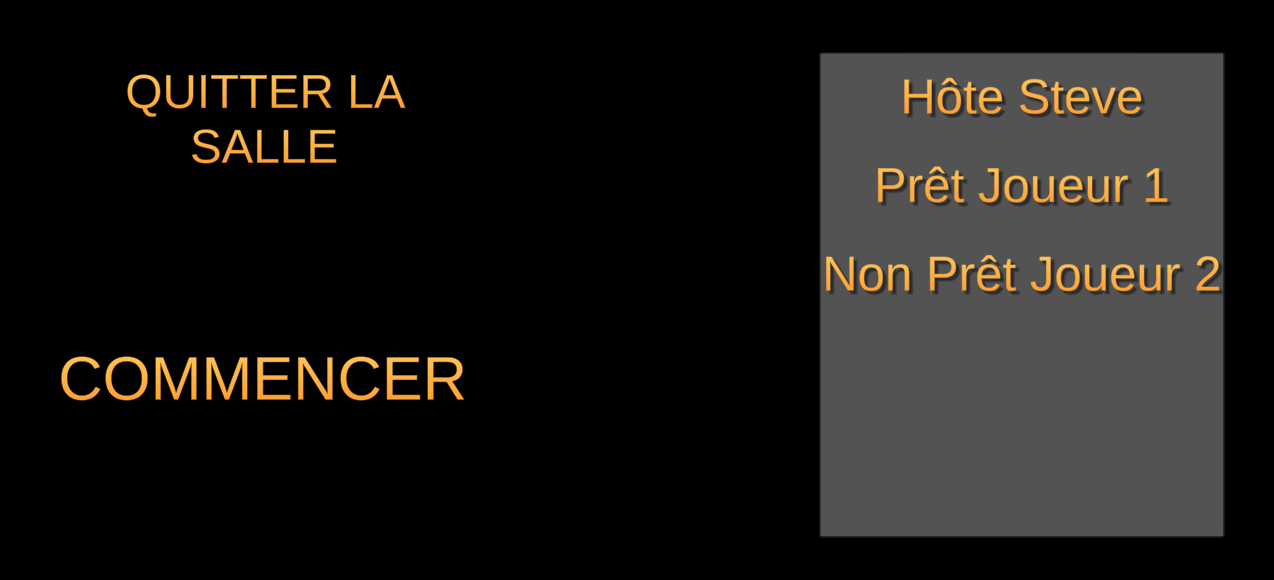
\includegraphics[width=0.8\textwidth]{Menu31.png}
    \caption{Menu lorsqu'on est hôte}
    \label{Menu lorsqu'on est hôte}
\end{figure}



\begin{figure}[!ht]
    \centering
    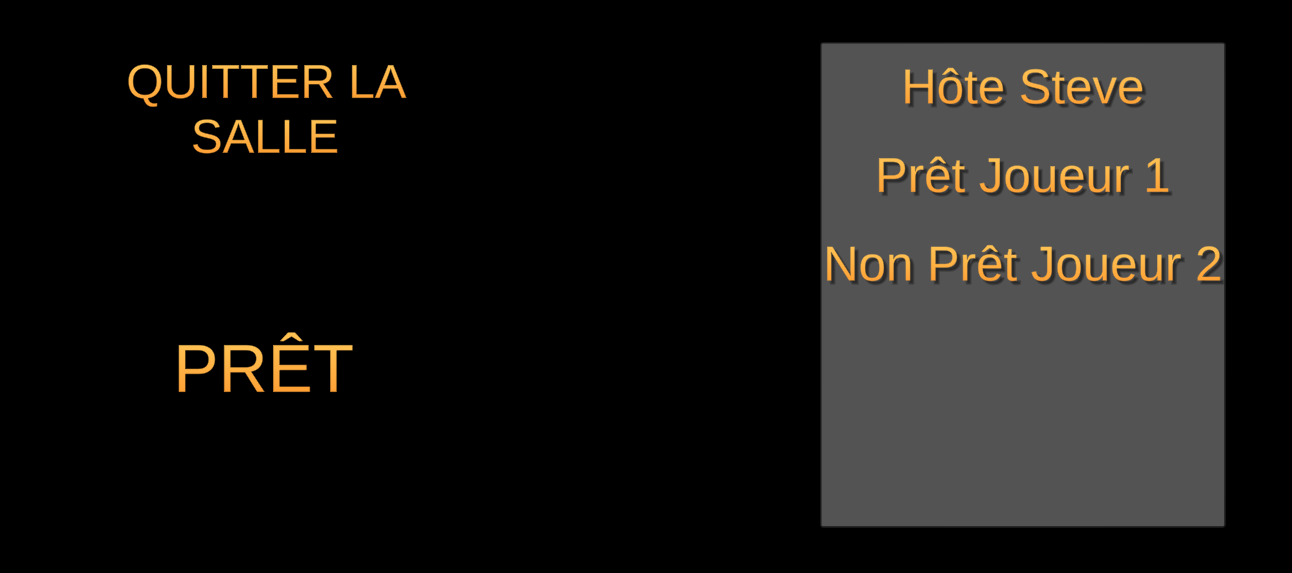
\includegraphics[width=0.8\textwidth]{Menu32.png}
    \caption{Menu lorsqu'on n'est pas hôte}
    \label{Menu lorsqu'on n'est pas hôte}
\end{figure}


\paragraph{Interface}
blablabla
\subsection{Gameplay}
blablabla
\subsubsection{Joueur}
%%%%%%%%%%%%%%%%%%%%%% Celian %%%%%%%%%%%%%%%%%%%%%%%%%%%%%%
blablabla
\subsubsection{Objets}
\paragraph{Génération d'Objets}
Etant donné que nous étions en avance sur nos prévisions de progression dans le projet, nous nous étions dis lors de la seconde soutenance que nous aurions peut-être le temps de rajouter quelques éléments qui ne figuraient pas dans le cahier des charges avant la dernière soutenance. C'est effectivement ce qu'il s'est passé. Nous avons donc décidé d'implémenter un système d'Objets récupérables au sein des laboratoires, afin d'aider les Joueurs ou, au contraire, de les gêner. Pour cela, j'ai tout d'abord réfléchi à l'implémentation des Objets. Un Objet doit remplir plusieurs critères. Premièrement, il ne doit jamais apparaître à l'intérieur d'un Sérum. Ensuite, il ne doit pas y avoir d'Objets à chaque salle du Labyrinthe. Pour ces deux raisons, nous ne pouvions pas mettre au point un système d'apparition d'Objets à intervalle de temps réguliers, car dans le cas où les Joueurs auraient peur des éventuels effets négatifs, le nombre d'Objets ne cesserait d'augmenter jusqu'à dépasser la contenance du labyrinthe, ce qui n'est absolument pas le but recherché. Finalement, nous avons décidé de faire en sorte que dans le Labyrinthe, il y aurait chaque fois un nombre constant d'Objets, Sérums compris. Ainsi, lorsqu'un Objet ou un Sérum est ramassé, il suffit juste d'évaluer une case ou un Sérum ou un autre Objet ne se trouve pas, et d'y générer le nouvel Objet. Ce système permet ainsi d'éviter un surplus d'Objet dans le labyrinthe, et de rendre la recherche des Objets relativement dynamique, puisqu'ils ont la possibilité de se renouveler à l'infini sans pour autant menacer la fluidité du jeu. 

\paragraph{Nombre d'Objets}
Au début de la partie, nous devons donc définir un nombre d'Objets de base. Il fallait bien sûr prendre en compte le nombre de Sérums nécessaires, mais également la taille du labyrinthe. En effet, dans un labyrinthe 20x20, s'il n'y a que trois Objets, en trouver relève du défi pur et dur. Nous avons donc choisi de faire en sorte qu'il y ait toujours un Objet par lot de 25 salles. Ainsi, un labyrinthe 10x10 aura quatre Objets, tandis qu'un labyrinthe 20x20 en comportera seize, ce qui est raisonnable étant donné qu'un dédale 20x20 est quatre fois plus grand qu'un dédale 10x10. De plus, j'ai pris soin de vérifier que pour le nombre, il y avait assez pour mettre suffisamment de Sérum au début de la partie. Si le nombre de salles est trop faible, j'augmente donc le nombre d'Objets pour qu'il y ait au moins le bon nombre de Sérums au début. Concernant l'apparence des Objets, vous aurez peut-être reconnu les cubes de Portal.

\paragraph{Sélection d'Objet}
Maintenant que les Objets sont implémentés, il faut leur ajouter des effets différents. Actuellement, il existe une douzaine d'effets différents. Il existe trois catégories d'effets, et deux sortes d'Objets. Les catégories sont : effets positifs, effets négatifs, et effets inutiles. Les Objets, eux, peuvent soit s'appliquer au moment où le Joueur les prend, soit rester sur le Joueur jusqu'à pouvoir être utilisés. Pour ces derniers, j'ai donc rajouté un tableau de booléens visant à déterminer si le Joueur a déjà les effets d'un Objet spécifique, et surtout d'afficher la liste de ces Objets sur son écran. Bien sûr, un Joueur ne peut pas récupérer un Objet qu'il a déjà. L'algorithme que j'ai utilisé choisit donc un des Objets parmi ceux que le Joueur peut potentiellement recevoir. Par exemple, si le Joueur est déjà équipé de Bottes de Pégase, il ne peut pas retomber sur des Bottes de Pégase à moins de les avoir perdues. De plus, certains Objets nécessitent de se trouver en seconde phase, et d'autres ne peuvent être pris que par un Joueur Guéri.

\paragraph{Image de la Carte}
Avant de commencer à faire de nombreux Objets, j'ai commencé par développer la Carte. En effet, j'avais pris soin de laisser le coin inférieur-gauche de l'écran en vue de cet Objet. Le problème, c'est qu'il n'y a qu'un seul joueur qui a accès au plan du Labyrinthe. Le Créateur de la Partie. J'ai donc réarrangé mon algorithme de construction de la carte. En effet, j'avais, lors de mes recherches pour la construction du labyrinthe, formulé deux versions : une par salle, qui est d'ailleurs utilisée pour générer le labyrinthe tel que vous le voyez maintenant, et une par bloc, qui permettait justement de comparer les plans des différents labyrinthes de manière très simple. Tout ce qu'il me restait à faire, c'était donc de transposer ces deux algorithmes pour construire à la fois le labyrinthe tridimensionnel et l'image renfermant la carte du labyrinthe. Ensuite, Steve et Célian se sont débrouillés pour faire en sorte que lorsque le Créateur du Salon envoie le message aux autres joueurs leur indiquant qu'ils peuvent générer leur personnage, il leur envoie également le Mode de jeu actuel, les dimensions du Labyrinthe, et la carte. Voici comment j'ai pu faire en sorte que tous les Joueurs aient accès à la Carte.

\paragraph{Affichage et Disparition de la Carte}
Concernant son affichage, il m'a fallu plus de temps. J'attendais de la Carte qu'en plus d'afficher le plan du complexe, elle affiche la position du Joueur la détenant en temps réel, afin de lui fournir de véritables indications. J'ai donc dû effectuer de nombreux tests, pour faire en sorte que la carte ne soit pas affichée au début dans un premier temps, puisque Unity affiche les images par défaut, et ensuite pour mettre au point le curseur sur la Carte, l'actualiser en fonction de la position du Joueur et le décaler en fonction de cette position et par rapport à la Carte. La difficulté, ici, est évidemment que l'affichage de la carte est simplifié et ne prend pas en compte la position exacte des murs. Autrement dit, affecter au Curseur une bête position directement proportionnelle aux coordonnées du Joueur ne suffit pas ; il me fallait plutôt déterminer la salle où le Joueur se trouvait. C'est cette partie qui m'a pris le plus de temps, car une erreur de quelques centimètres peut afficher le Joueur de l'autre côté d'un mur qu'il n'a pourtant pas franchi. Mais heureusement, tout fonctionne actuellement à merveille. J'ai également pris soin de laisser une fonction permettant d'effacer la Carte au besoin.

\paragraph{Objets de base}
Une fois que la Carte a été achevée, je suis alors passé au développement de cinq Objets basiques. Les Bottes de Pégase, qui donne au Joueur une vitesse deux fois plus importante que la normale, les Bottes de Plomb, qui lui donnent au contraire une vitesse deux fois moins importante que la normale, la Carte, qui affiche évidemment la Carte, la Paralysie, qui l'immobilise un faible instant, et la Décharge, qui lui retire tous les Objets qu'il conserve sur lui. Il y avait donc trois Objets à effets constants et deux à effets immédiats. Pour les Bottes de Pégase et les Bottes de Plomb, il m'a suffit d'affecter une valeur à un ratio de vitesse que Célian avait laissé comme propriété sur les Joueurs. Pour la Carte, je n'avais plus qu'à lancer la fonction d'affichage de cette dernière, et pour la Paralysie, à baisser la valeur "Stamina" à 0, pour simuler le choc lorsqu'un autre Joueur vout frappe. Pour la Décharge, il me suffisait donc de mettre à false tous les éléments du tableau des Objets constants, de lancer la fonction annulant l'affichage de la carte, et de rétablir la vitesse à son ratio normal. Bien sûr, comme indiqué précédemment, un Joueur ne peut pas prendre de Bottes de Pégase s'il en a déjà sur lui. Cela dit, j'ai fait en sorte que le Joueur puisse récupérer des Bottes de Plomb lorsqu'il a les Bottes de Pégase, et ainsi de suite. L'Objet ainsi récupéré devient alors tout de suite effectif, au lieu de simplement rétablir la vitesse du Joueur à sa vitesse normale. Autrement dit, si vous avez les Bottes de Plomb et que vous récupérez des Bottes de Pégase, vous avancerez quatre fois plus vite par rapport à la vitesse que vous aviez. J'ai également fait attention à ce que les Objets du Joueur se réactualisent à chaque fois qu'il prend un Objet.

\paragraph{Deuxième vague d'Objets}
Suite à ces cinq Objets, je me suis lancé dans la confection de trois autres Objets de cet acabit : la Disparition, la Protection, et le Casque de CRS. Ces trois Objets sont à effets constants. La Protection a un effet très simple, elle permet d'annuler l'effet d'un Objet à effet négatif. Il s'agit donc juste d'un effet à prendre en compte lors de l'application des effets des différents Objets. La Disparition, elle, permet à un joueur Guéri en seconde phase de devenir invisible pendant quinze secondes. Il devient alors inconsistant : il ne peut être infecté durant ce labs de temps, mais il ne peut pas non plus prendre d'Objets. Le Casque de CRS, lui, dissimule le labyrinthe au Joueur, qui doit donc avancer à l'aveuglette pendant quinze secondes, le temps de retirer le Casque. Ces deux Objets m'ont donné plus de fil à retordre que les autres. En effet, je souhaitais faire en sorte que les quinze secondes puissent être interrompues, avec l'effet qui cesse, en vue de la Décharge. Evidemment, ce n'était pas nécessaire pour la Disparition, mais plus pour le Casque de CRS. 

\paragraph{Développement d'un chronomètre désactivable}
Pour cela, j'ai fait en sorte que le "chronomètre" soit constitué d'un entier indiquant le temps restant en seconde et d'un booléen indiquant si une seconde était en train d'être comptée. Ainsi, à chaque image du jeu, je vérifiais que la seconde aie terminé d'être comptée. Si c'était le cas, je relançais une seconde, sinon je ne faisais rien. Et ainsi de suite, jusqu'à ce que le nombre de secondes tombe à 0. Dans ce cas, je lançais automatiquement l'arrêt de l'effet. Ainsi, pour désactiver un Casque de CRS quand on se prend une Décharge, il suffit simplement de baisser le nombre de secondes restantes à 0. De plus, quand le compteur passe à 0, je prenais soin de retirer l'Objet en question du tableau des Objets du Joueur, et de remettre à jour l'affichage de ces valeurs à l'écran. Concernant le Casque de CRS, j'avais également voulu le faire au départ un simple affichage de rectangle noir avec la propriété OnGUI de Unity. Le soucis, c'est qu'avec cette méthode, on ne voyait ni le nom du Joueur, ni son état, ni le temps qu'il restait avant la fin de la Partie, ni la Carte s'il l'avait, ni le message comme quoi le Joueur avait reçu le Casque de CRS, ni la liste des Objets que le Joueur avait. J'ai donc dû me résoudre à utiliser une Image, pour pouvoir la reléguer en arrière-plan, entre l'image du dédale et les différents éléments constituant l'écran du Joueur. J'ai ensuite dû faire en sorte que l'affichage noir lié à la présence automatique du Casque par Unity disparaisse au début du jeu pour chaque Joueur. On en est donc à huit Objets.

\paragraph{Dernière vague d'Objets}
Les cinq Objets restants, je les ai implémenté avec plus de facilité que les précédents. Il s'agit du Champignon, du Sérum d'Urgence, de l'Herbe Bleue, du Catalyseur et des Ressorts. Le Champignon et les Ressorts sont des Objets Inutiles : le Champignon vous assène simplement des sons particuliers dans votre oreillette, à la manière d'hallucinations sonores, et les Ressorts vous font sauter automatiquement pendant quelques secondes. Etant donné que je savais déjà comment évaluer ce type de chronomètre, les Ressorts ont été relativement simples à encoder. Pour le Champignon, j'ai en revanche dû m'arranger avec Célian pour comprendre la manière dont il avait inséré les sons dans le programme. Le Catalyseur, lui, est un Objet à effet négatif qui reste jusqu'à ce que vous vous preniez une Décharge : il double tout simplement le temps de récupération après une Paralysie, que ce soit déclenché par l'Objet Paralysie ou par un autre Joueur. Quant au Sérum d'Urgence et à l'Herbe Bleue, ils ont été plus intéressants à développer. Pour commencer, ces deux Objets ne peuvent être récupérés qu'en seconde phase. Le premier, en plus, ne peut être pris que par un Joueur Guéri. Le Sérum d'Urgence permet à un Joueur Guéri de disparaître quand il se fait infecté. Autrement dit, quand un Joueur Condamné effleure le Joueur Guéri ayant ce Sérum d'Urgence, il a la surprise de voir ce Joueur disparaître au lieu de devenir simplement un nouveau Condamné. Le Joueur qui vient de disparaître, quant à lui, dispose de cinq secondes avant de redevenir visible, et donc de nouveau infectable. On peut donc considérer qu'il s'agisse d'une vie supplémentaire.

\paragraph{L'Herbe Bleue, un Objet Commun}
L'Herbe Bleue, elle, est un Objet Commun. Autrement dit, quand un Joueur ramasse une Herbe Bleue, l'effet s'applique sur tout le monde. En effet, l'Herbe Bleue rallonge de trente secondes la durée de la seconde phase. Pour implémenter ces deux Objets, il m'a donc fallu comprendre où se déroulait l'infection d'un Joueur, et faire en sorte de pouvoir rallonger le temps de la seconde phase tout en affichant un message aux autres Joueurs pour les prévenir de ce détail. Pour le Sérum d'Urgence, j'ai donc regardé du côté de la fonction que Célian utilisait pour faire changer un Joueur d'état. Dans le cas où le nouvel état était l'état de Condamné, il m'a donc suffit de rajouter la condition de la présence du Sérum d'Urgence dans les Objets de Joueur en question. S'il en avait un, il ne me restait plus qu'à faire en sorte que l'état dans lequel il serait serait l'état d'invisible au lieu de Condamné, et de lancer en même temps un chronomètre de cinq secondes pour rétablir l'état Guéri du Joueur plus tard. J'ai procédé de la même manière pour l'Herbe Bleue : j'ai rendu la variable des chronomètres de seconde phase des Joueurs directement accessible via le script PlayerNetwork, où sont effectuées la majorité des fonctions en réseau. Ainsi, quand quelqu'un reçoit une Herbe Bleue, il lui suffit de lancer la fonction en réseau correspondante. Et quand un Joueur reçoit cette fonction, le chronomètre augmente de trente secondes. Avec, bien sûr, un petit message sur son écran dans le cas où il ne s'agirait pas du Joueur ayant récupéré ledit Objet.

\subsection{Labyrinthe}
blablabla
\subsubsection{Partie de Léandre}

\paragraph{Génération aléatoire du Labyrinthe}
Au début du projet, il a été décidé que je serais le responsable de l'ensemble des éléments aléatoires du jeu, ainsi que de la direction artistique. J'ai ainsi commencé en mettant au point un algorithme permettant de générer un dédale de telle sorte que l'ensemble des salles soit accessibles, et que pour accéder à une salle à partir d'un endroit du labyrinthe, il y ait plusieurs itinéraires. L'algorithme a été développé en faisant en sorte qu'il n'y ait aucune sortie, et que l'on puisse modifier la taille du labyrinthe. Au final, l'algorithme correspond à peu de choses près à l'algorithme de Prim, excepté le fait que le nombre d'impasse est nettement moins important. A côté de cette fonction, j'ai également créé une seconde fonction retournant une liste d'entiers aléatoires distincts dans un intervalle donné.

\paragraph{Labyrinthe en Cubes}
A partir de cet algorithme, on obtient donc une liste dont les valeurs correspondent directement aux passages de chaque "case" du labyrinthe. Pour vérifier que l'algorithme fonctionnait bien, et vite, j'ai mis au point une petite fonction qui se charge d'afficher la carte du labyrinthe ainsi formé dans une console. Après de nombreux tests, aucours desquels j'ai modifié la taille du dédale pour obtenir des configurations rectangulaires, cubiques, voire linéaires pour vérifier le bon fonctionnement de l'algorithme, j'ai transposé le tout sur Unity. J'ai alors modifié la fonction d'affichage en faisant en sorte qu'à la place de mettre des caractères dans une console, Unity instancie des cubes dans une "Scène" prévue à cet effet.

\paragraph{Labyrinthe en Salles}
Ensuite, étant donné que nous souhaitions donner à l'ensemble une structure évoquant plus un laboratoire souterrain qu'un jeu de cube pour enfants, j'ai développé une autre fonction pour afficher non pas les murs séparément, mais directement des modèles 3D de salles avec les passages, pour simuler un vrai labyrinthe. La difficulté était ici de bien configurer pour chaque salle l'orientation, ainsi que la position au sein du labyrinthe. Mais j'ai tout de même conservé l'affichage en bloc en vue d'autres tests de génération de l'algorithme, étant donné que cet affichage permet de vérifier plus aisément que la carte du labyrinthe soit valable. Les modèles 3D que j'ai utilisé étaient surtout là pour simuler la carte dans un labyrinthe, et pour effectuer des tests en multijoueur.

\paragraph{Labyrinthe et Sérums}
A partir de là, on obtient donc un labyrinthe correct, bien que dénué de décorations évoquant un laboratoire. Mais bien qu'il y ait un format correct, ce n'était pas encore jouable : il manquait bien sûr les Sérums et les Joueurs. Concernant les Joueurs, Célian a implémenté une rampe permettant de monter pour sauter directement dans le complexe. En revanche pour les sérums, il nous fallait prendre en compte plusieurs facteurs. Premièrement, un Sérum ne devait pas être implémenté à l'intérieur d'un autre Sérum. Deuxièmement, un Joueur ne devait pas être instancié au même emplacement qu'un Sérum, pour éviter qu'un Joueur ne se retrouve infecté dès le début de la partie. Pour cela, j'ai réutilisé la fonction permettant d'obtenir une liste d'entiers aléatoires distincts. Avec cette fonction, il m'était en effet possible d'isoler sept "cases" du complexe dans lesquelles seraient respectivement implémentés les quatres joueurs et les trois sérums. Ainsi, au lancement du jeu, j'ai fait en sorte que le joueur génère les sérums à l'emplacement souhaité. Pour les Sérums, nous n'avions alors que des cubes mauves pour les représenter. 

\paragraph{Labyrinthe en Réseau}
Restait alors la question de l'initialisation du labyrinthe en réseau. La difficulté était alors de faire en sorte que chaque joueur ait la même carte, et que les Sérums réagissent en réseau. Concernant ce second point, il nous est apparu nécessaire que les sérums, ainsi que les positions des joueurs et la carte du dédale, soient générés par un seul joueur. Le Joueur le plus reconnaissable en réseau étant le Créateur de la Partie, j'ai donc rajouté une condition à la génération du labyrinthe pour faire en sorte que le Créateur du Salon soit le seul à être en mesure de construire le labyrinthe, en instanciant des objets Photon en réseau. Le processus marchait bien pour la génération avec l'affichage en blocs, pour les murs et les Sérums. Mais nous avons rencontré quelques difficultés avec l'affichage en salles. En effet, dans la Partie du Créateur de la Partie, tout se générait correctement. Mais concernant les autres joueurs, nous nous sommes vite rendus compte que les salles étaient toujours orientées dans le même sens. Ce n'est qu'après coup que nous avons réalisé que le problème venait du fait que Photon n'enregistrait pas les rotations de salles effectuées par le Créateur du Salon. Nous avons rapidement corrigé ce détail, et après cela, nous avons pu commencer à effectuer des semblants de partie dans le labyrinthe, même si la seconde phase ne se lançait pas encore.

\paragraph{Répartion des Joueurs}
Le prochain objectif concernant la génération de la partie était alors de faire en sorte que les Joueurs apparaissent à des endroits différents dans le labyrinthe. Avant de commencer à nous attaquer directement à l'aléatoire, nous avons décidé de faire en sorte que les joueurs apparaissent sur quatre socles à l'extérieur du dédale. Après de nombreux essais, Steve a remarqué que via Photon, les Joueurs n'apparaissaient pas tous en même temps, mais les uns après les autres. Il s'est alors appuyé sur ce détail pour distinguer les Joueurs avec leur arrivée dans la Partie, en prenant en compte le nombre de Joueurs déjà présents. Effectivement, grâce à ce procédé, nous avons réussi à faire en sorte que les joueurs ne puissent pas apparaître au même endroit. Mais en utilisant cette méthode avec les quatres entiers prédéfinis pour les positions des joueurs dans le labyrinthe, nous nous sommes très vite rendus compte qu'il y avait une faille dans notre procédé. En effet, rien ne garantissait que le Master soit instancié en premier, ce qui faisait que souvent, les joueurs qui avaient le malheur d'apparaître avant lui se retrouvaient les genoux dans le sol. Steve a alors rajouté une option permettant de faire en sorte que le Créateur de la Partie soit le premier Joueur à être instancié, et envoit un message aux autres joueurs pour qu'ils puissent le rejoindre dans le labyrinthe. A partir de là, nous avons pu commencer à simuler de véritables débuts de partie.

\paragraph{Un décor de laboratoire}
Avec Yann, nous nous sommes alors appliqué à donner à l'ensemble un aspect beaucoup plus agréable que les modèles 3D rose vif et vert clair que nous utilisions. Nous nous sommes donc intéressé à Blender. J'ai commencé par créer un modèle pour les Sérums plus digne d'un véritable laboratoire qu'un bête cube tout droit sorti d'une caisse de jouets pour enfants. Puis nous nous sommes concentrés sur les salles. Nous avons commencé par déterminer les différents types de salle que l'on peut croiser dans un laboratoire : des salles de stockage, des salles d'information, des salles d'expérimentation, des couloirs, des salles de réflexion et des serres. Nous avons ensuite réparti ces catégories de salles en fonction de la probabilité d'avoir un certain nombre de portes, afin de les rétablir équitablement entre les différentes salles du labyrinthe. Ainsi, les salles de stockage n'ont qu'une porte et forment des impasses, les salles d'information en ont quatre et correspondent à des croisements, les salles d'expérimentations en ont deux et forment respectivement un couloir droit et un couloir tournant, et les couloirs classques et les salles de réflexion, elles ont trois portes, il s'agit donc d'embranchements.

\paragraph{De nouveaux modèles 3D}
Je me suis ainsi occupé des serres, des salles d'expérimentation et des couloirs, tandis que Yann s'occupait des salles de réflexion, des salles d'information et des salles de stockage. Nous avons ainsi produit des modèles 3D à partir de Blender, que nous avons ensuite inséré à la place des modèles roses des précédentes version du labyrinthe. Nous avons fait attention à ce que les portes n'aient pas de rebords bloquants, afin de permettre aux Joueurs de courir plus aisément à l'intérieur du dédale. Cependant, nous avons eu un problème avec les salles d'information ; en effet, à la base, Yann avait prévu de mettre quatre écrans reliés avec un câble pendant du plafond. Le problème se posait pour les Joueurs et pour les Sérums : si un Sérum apparaissait dans ce type de salle, les écrans le rendaient inaccessible. De même, un joueur apparaissant dans cette salle se retrouvait bloqué par le câble au plafond, étant donné que les Joueurs arrivent du dessus du dédale. Nous avons donc modifié la configuration de manière à laisser l'accès libre au centre de la pièce. A côté de ça, il restait encore trois détails à régler pour la génération complète du labyrinthe : le mobilier, les salles d'attente où apparaissent dans un premier temps les Joueurs, et les lumières.

\paragraph{Luminosité}
Concernant le mobilier, je me suis appliqué à mettre des chaises, des ustensiles, des fioles, des plantes et des feuilles dans les modèles 3D, afin de donner l'impression qu'il s'agisse d'un véritable lieu de travail. De plus, je me suis amusé à glisser des références à d'autre jeux dans le décor. Peut-être aurez-vous l'occasion de les découvrir ? Mais qu'importe. Pour les salles d'attente, j'ai préféré faire en sorte que chaque joueur initialise sa propre salle en réseau, plutôt que de laisser au Créateur de la Partie le soin de tout charger. La décoration de ces salles est nulle, il s'agit juste de dissimuler l'extérieur du labyrinthe en attendant que tout les joueurs soient instanciés, afin de les faire commencer en même temps. Le seul élément distinctif est un trou dans le sol, qui permet de faire tomber le Joueur dans les méandres du dédale des souterrains du laboratoire. Enfin, concernant les lumières, j'ai créé un autre modèle 3D, un plafond, avec une lampe. La couleur de cette lampe est modulable directement via une fonction, ce qui permet entre autre de modifier sa couleur. Afin d'assurer le meilleur rendu possible, nous avons décidé de mettre les lumières en qualité importante, afin d'éviter les problèmes d'ombres entre les différents éléments du dédale. J'ai également prit soin de surélever le plafond si la salle était destinée à accueillir un Joueur. Enfin, j'ai annulé la luminosité ambiante de la Scène Unity. 

\paragraph{Mode Nocturne}
Le rendu est beaucoup plus réaliste que ce que nous avions précédemment. Cela dit, les lumières sont coûteuses en puissance. Pour éviter des problèmes avec Photon, nous avons décidé de limiter le nombre de salles possibles dans un labyrinthe à seulement 400. De plus, j'ai eu l'idée d'implémenter un second mode de jeu. Il s'agit du mode "NOCTURNE". Comme son nom l'indique, ce mode permet au Joueur de se retrouver dans un labyrinthe plongé dans le noir. L'unique lumière venant alors des joueurs, ce mode peut changer la donne, puisqu'il devient dès lors très difficile de se cacher. De même, à moins qu'il n'y ait un joueur devant soi, il est très dur de deviner les salles se trouvant devant le joueur actuel, ou même s'il y a un Sérum devant soi. Ce mode est donc beaucoup plus plaisant à jouer, non seulement pour l'ambiance beaucoup plus prenante que dans le mode "CLASSIQUE", mais également parce que les éventuels ralentissements dûs à un effort de l'ordinateur pour les lumières ne sont plus du tout présents. Un autre détail concernant les lumières est que j'ai fait en sorte que lorsque l'on passe en seconde phase et que l'on est en mode "CLASSIQUE", les lumières des lampes, jusque là blanches, deviennent rouges, afin d'évoquer de manière plus concrète une alarme de laboratoire.

%%%%%%%%%%%%%%%%%%%%%% Steve%%%%%%%%%%%%%%%%%%%%%%%%%%%%%%

\subsection{Réseau}
blablabla
\subsection{Site Web}
blablabla
%%%%%%%%%%%%%%%%%%%%%% Yann %%%%%%%%%%%%%%%%%%%%%%%%%%%%%%
\subsection{Sons et musiques}
blablabla
\subsubsection{Sons}
blablabla
\subsubsection{Musiques}
\paragraph{Première tentative}
Pour travailler sur les musiques du jeu, j'ai utilisé un logiciel de partition nommé MuseScore, qui, en plus d'être gratuit, permet de générer directement une partition complète avec de nombreux instruments, et d'exporter la piste sonore en fichier MIDI. J'ai commencé dans un premier temps à faire plusieurs essais d'ambiance pour le thème de la Recherche de Sérum. Je tenais à rendre l'atmosphère assez stressante. Pour cela, j'ai utilisé un violon qui émet une note à intervalles précis et réguliers, à la manière d'une alarme d'évacuation. J'ai ensuite rajouté une percussion pour renforcer l'ambiance pesante et lourde, tout comme la contrebasse qui se charge du thème. Ensuite, Célian a remixé la piste obtenue, et le résultat est celui que vous pouvez entendre à vos oreilles en lançant une nouvelle partie.

\paragraph{Autres thèmes}
Ensuite, j'ai commencé à faire le thème du Menu Principal. Ici, je tenais à rendre l'atmosphère plutôt pesante et inquiétante. J'ai donc inséré en fond un piano qui répète la même note à la manière d'un tictac d'horloge, accompagné d'un trombone qui se charge de la basse. Enfin, j'ai également composé deux mélodies, l'une pour la victoire, la seconde pour la mort du joueur. Pour la première, j'ai cherché à faire quelque chose d'assez joyeux et léger, tandis que pour l'autre, j'ai utilisé des instruments beaucoup plus graves ainsi que des notes plus longues pour accentuer le sentiment de deuil. Tout comme pour la musique de la recherche de sérums, c'est Célian qui s'est chargé de remixer le tout, en modifiant notamment l'instrumentation. Actuellement, le jeu possède donc quelques musiques originales. Le problème, c'est que... Ce n'est pas dit que beaucoup de personnes apprécient. Mais au moins, il n'y aura pas de soucis avec les droits d'auteurs !

%%%%%%%%%%%%%%%%%%%%%% Léandre %%%%%%%%%%%%%%%%%%%%%%%%%%%%%%
%%%%%%%%%%%%%%%%%%%%%% Celian %%%%%%%%%%%%%%%%%%%%%%%%%%%%%%

\newpage
\section{Réalisations}
blablabla
\subsection{Nos joies}
blablabla
\subsection{Nos peines}
blablabla
\newpage
\section{Conclusion}

%%%%%%%%%%%%%%%%%%%%%%%%%%%%%% TODO : Mettre a jour

\emph{If you knew time as well as I do, you would play Deadly Science.}


\end{document}



